\providecommand{\dD}{\mathrm{d}}
%% ---------------- figures (TikZ redraws of the answer-sheet graphs)
\newcommand{\figRIcurrent}{\begin{tikzpicture}[x=1.1cm,y=1.6cm,font=\small]
\draw[->,thick](-0.2,0)--(8,0) node[right]{$t$};\draw[->,thick](0,-0.2)--(0,1.7) node[above]{$I$};
\draw[blue!70!black,semithick,domain=0:7.8,samples=80] plot(\x,{2.718*\x*exp(-2*\x/3)/1.5});
\fill (1.5,1) circle(1.5pt) node[above right]{$\left(\dfrac32,\dfrac{3A}{2\mathrm{e}}\right)$};
\node[below left] at (0,0){$O$};
\end{tikzpicture}}
\newcommand{\figNJCpressure}{\begin{tikzpicture}[x=0.075cm,y=0.022cm,font=\small]
\draw[->,thick](-3,0)--(95,0) node[right]{$h$};\draw[->,thick](0,-8)--(0,140) node[above]{$P$};
\draw[semithick,domain=0:88,samples=120] plot(\x,{101.3*((abs(293-6.5*\x)/293)^5.2015)});
\node[left] at (0,101.3){$101300$};\node[below left] at (0,0){$O$};\node[below] at (45.1,0){$45.1$};
\end{tikzpicture}}
%% ============================================================ 131 HCI 2025 Prelim P1 Q10 (soln: HCI_2025_H2_Math_Prelim_P1_Solutions.pdf pp16-18, official)
\defQ{131}{}{%
\begin{qparts}
\pt{(a)} Express $\dfrac{1}{Q\left(500-Q\right)}$ in partial fractions. \mk{2}
\pt{(b)} A group of scientists is monitoring the population of a particular species of birds on an island. At time $t$ years after the start of the monitoring, the number of birds on the island is $Q$. The scientists observe that the birth rate is proportional to the bird's population and the birds are dying at a rate proportional to the square of the bird's population. There were 1000 birds on the island when the scientists first started monitoring the population. They discover that the population remains unchanged when there are 500 birds.
\begin{qparts}
\pt{(i)} Show that the differential equation relating $Q$ and $t$ is given by
\[\frac{\dD Q}{\dD t}=kQ\left(500-Q\right),\]
where $k$ is a positive constant. \mk{2}
\pt{(ii)} Hence, solve the differential equation, expressing $Q$ in terms of $k$ and $t$. \mk{5}
\end{qparts}
\end{qparts}
\src{HCI 2025 Prelim P1 Q10}}
\defS{131}{%
\begin{gtpart}{(a)}{2}\begin{topalign}
\frac{1}{Q\left(500-Q\right)}&=\frac{A}{Q}+\frac{B}{500-Q}=\frac{\left(500-Q\right)A+BQ}{Q\left(500-Q\right)}\\
\Rightarrow1&=A\left(500-Q\right)+BQ
\end{topalign}
For $Q=0$, $1=500A\Rightarrow A=\dfrac{1}{500}$.\par
For $Q=500$, $1=500B\Rightarrow B=\dfrac{1}{500}$.
\begin{topalign}
\therefore\frac{1}{Q\left(500-Q\right)}&=\frac{1}{500Q}+\frac{1}{500\left(500-Q\right)}
\end{topalign}\end{gtpart}
\begin{gtpart}{(b)(i)}{2}Increase rate $\propto Q$\par
$\Rightarrow$ Increase rate $=aQ$ ($a$ is the constant of proportionality for increase rate)\par\smallskip
Decrease rate $\propto Q^{2}$\par
$\Rightarrow$ \fhl{Decrease rate} $=bQ^{2}$ ($b$ is the constant of proportionality for decrease rate)
\begin{topalign}
\therefore\frac{\dD Q}{\dD t}&=aQ-bQ^{2}\quad\text{(Increase rate -- Decrease rate)}
\end{topalign}
$\dfrac{\dD Q}{\dD t}=0$ when $Q=500$
\begin{topalign}
\Rightarrow500a-250000b&=0\\
\Rightarrow a&=500b\\
\therefore\frac{\dD Q}{\dD t}&=500bQ-bQ^{2}\\
\Rightarrow\frac{\dD Q}{\dD t}&=kQ\left(500-Q\right)\quad\text{where }k=b
\end{topalign}\end{gtpart}
\begin{gtpart}{(b)(ii)}{5}\begin{topalign}
\int\frac{1}{Q\left(500-Q\right)}\,\dD Q&=\int k\,\dD t\\
\frac{1}{500}\int\frac1Q+\frac{1}{500-Q}\,\dD Q&=\int k\,\dD t\quad\text{(from part (a))}\\
\frac{1}{500}\Big[\ln Q-\ln\left|500-Q\right|\Big]&=kt+C\\
\ln\left|\frac{Q}{500-Q}\right|&=500kt+500C
\end{topalign}
\textbf{Resolving the modulus}:\par\smallskip
\underline{\textbf{Method 1 (using arbitrary constant):}}
\begin{topalign}
\ln\left|\frac{Q}{500-Q}\right|&=500kt+500C\\
\Rightarrow\left|\frac{Q}{500-Q}\right|&=\mathrm{e}^{500kt+500C}\\
\Rightarrow\frac{Q}{500-Q}&=\pm\mathrm{e}^{500C}\mathrm{e}^{500kt}\\
\Rightarrow\frac{Q}{500-Q}&=H\mathrm{e}^{500kt},\quad\text{where }H=\pm\mathrm{e}^{500C}\text{ is an arbitrary constant}
\end{topalign}
Therefore, we have
\begin{topalign}
Q&=500H\mathrm{e}^{500kt}-QH\mathrm{e}^{500kt}\\
Q&=\frac{500H\mathrm{e}^{500kt}}{1+H\mathrm{e}^{500kt}}
\end{topalign}
When $t=0$, $Q=1000$
\begin{topalign}
\frac{1000}{500-1000}&=H\Rightarrow H=-2\\
\therefore Q&=\frac{-1000\mathrm{e}^{500kt}}{1-2\mathrm{e}^{500kt}}\\
\Rightarrow Q&=\frac{1000\mathrm{e}^{500kt}}{2\mathrm{e}^{500kt}-1}
\end{topalign}
\underline{\textbf{Method 2 (using the initial condition):}}\par
When $t=0$, $Q=1000$, and $Q$ stabilized at 500 given in the question.\par
Therefore $Q\geq500\Rightarrow Q-500\geq0$
\begin{topalign}
\Rightarrow\ln\left|\frac{Q}{500-Q}\right|&=\ln\left(\frac{Q}{Q-500}\right)
\end{topalign}
Hence we have
\begin{topalign}
\ln\left(\frac{Q}{Q-500}\right)&=500kt+500C=500kt+D
\end{topalign}
When $t=0$, $Q=1000$
\begin{topalign}
\ln\left(\frac{1000}{1000-500}\right)&=0+D\\
\Rightarrow D&=\ln2\\
\ln\left(\frac{Q}{Q-500}\right)&=500kt+\ln2\\
\frac{Q}{Q-500}&=\mathrm{e}^{500kt+\ln2}\\
\frac{Q}{Q-500}&=\mathrm{e}^{\ln2}\mathrm{e}^{500kt}=2\mathrm{e}^{500kt}\\
Q&=2\mathrm{e}^{500kt}\left(Q-500\right)\\
Q-2\mathrm{e}^{500kt}Q&=-1000\mathrm{e}^{500kt}\\
Q&=\frac{-1000\mathrm{e}^{500kt}}{1-2\mathrm{e}^{500kt}}\\
Q&=\frac{1000\mathrm{e}^{500kt}}{2\mathrm{e}^{500kt}-1}
\end{topalign}\end{gtpart}}
%% ============================================================ 132 HCI 2025 Prelim P1 Q3 (soln: HCI_2025_H2_Math_Prelim_P1_Solutions.pdf p4, official)
\defQ{132}{}{%
It is given that $\left(2xy\dfrac{\dD y}{\dD x}+y^{2}\right)\cos x=\dfrac{1}{xy^{2}}$, where $0<x<\dfrac{\pi}{2}$ and $y\neq0$.
\begin{qparts}
\pt{(a)} Using the substitution $u=xy^{2}$, show that the differential equation can be reduced to $\dfrac{\dD u}{\dD x}=\dfrac{\sec x}{u}$. \mk{3}
\pt{(b)} Hence find the general solution to the differential equation. \mk{3}
\end{qparts}
\src{HCI 2025 Prelim P1 Q3}}
\defS{132}{%
\begin{gtpart}{(a)}{3}\begin{topalign}
u&=xy^{2}\\
\frac{\dD u}{\dD x}&=y^{2}+x\left(2y\frac{\dD y}{\dD x}\right)\\
\cos x\left(y^{2}+2xy\frac{\dD y}{\dD x}\right)&=\frac{1}{xy^{2}}\\
\cos x\left(\frac{\dD u}{\dD x}\right)&=\frac1u\\
\frac{\dD u}{\dD x}&=\frac{\sec x}{u}
\end{topalign}\end{gtpart}
\begin{gtpart}{(b)}{3}\begin{topalign}
\int u\,\dD u&=\int\sec x\,\dD x\\
\frac12u^{2}&=\ln\left(\sec x+\tan x\right)+C\quad\left(\because\sec x,\tan x>0\text{ for }0<x<\frac{\pi}{2}\right)\\
x^{2}y^{4}&=2\ln\left(\sec x+\tan x\right)+\fhlmi{D}
\end{topalign}\end{gtpart}}
%% ============================================================ 133 2018 A-level P1 Q10 (soln: Raffles Institution "Solution for 2018 A-Level Paper 1" pp10-11, grail.moe/library/9387; question paper not obtainable)
\defQ{133}{}{%
\fhlp{An electrical circuit comprises a power source of $V$ volts in series with a resistance of $R$ ohms, a capacitance of $C$ farads and an inductance of $L$ henries. The current in the circuit, $t$ seconds after turning on the power, is $I$ amps and the charge on the capacitor is $q$ coulombs. The circuit can be used by scientists to investigate resonance, to model heavily damped motion and to tune into radio stations on a stereo tuner. It is given that $R$, $C$ and $L$ are constants, and that $I=0$ when $t=0$.}\par\smallskip
\fhlp{A differential equation for the circuit is $L\dfrac{\dD I}{\dD t}+RI+\dfrac{q}{C}=V$, where $I=\dfrac{\dD q}{\dD t}$.}
\begin{qparts}
\pt{(i)} \fhlp{Show that, under certain conditions on $V$ which should be stated,
\[L\dfrac{\dD^{2}I}{\dD t^{2}}+R\dfrac{\dD I}{\dD t}+\dfrac{I}{C}=0.\]} \mk{2}
\end{qparts}
\fhlp{It is now given that the differential equation in part (i) holds for the rest of the question.}
\begin{qparts}
\pt{(ii)} \fhlp{Given that $I=At\mathrm{e}^{-\frac{Rt}{2L}}$ is a solution of the differential equation, where $A$ is a positive constant, show that $C=\dfrac{4L}{R^{2}}$.} \mk{5}
\pt{(iii)} \fhlp{In a particular circuit, $R=4$, $L=3$ and $C=0.75$. Find the maximum value of $I$ in terms of $A$, showing that this value is a maximum.} \mk{4}
\pt{(iv)} \fhl{Sketch the graph of $I$ against $t$.} \mk{2}
\end{qparts}
\src{2018 A-level P1 Q10}}
\defS{133}{%
\begin{gtpart}{}{}\begin{topalign}
L\frac{\dD I}{\dD t}+RI+\frac{q}{C}&=V,\quad\text{where }I=\frac{\dD q}{\dD t}
\end{topalign}\end{gtpart}
\begin{gtpart}{(i)}{}Differentiate with respect to $t$,
\begin{topalign}
L\frac{\dD^{2}I}{\dD t^{2}}+R\frac{\dD I}{\dD t}+\frac1C\frac{\dD q}{\dD t}&=\frac{\dD V}{\dD t}\\
L\frac{\dD^{2}I}{\dD t^{2}}+R\frac{\dD I}{\dD t}+\frac{I}{C}&=\frac{\dD V}{\dD t},\quad\text{since }I=\frac{\dD q}{\dD t}
\end{topalign}
Therefore,
\begin{topalign}
L\frac{\dD^{2}I}{\dD t^{2}}+R\frac{\dD I}{\dD t}+\frac{I}{C}&=0,\quad\text{when }\frac{\dD V}{\dD t}=0\text{ that is, }V\text{ is a constant.}
\end{topalign}\end{gtpart}
\begin{gtpart}{(ii)}{}\begin{topalign}
I&=At\mathrm{e}^{-\frac{Rt}{2L}}\\
\frac{\dD I}{\dD t}&=A\mathrm{e}^{-\frac{Rt}{2L}}+At\mathrm{e}^{-\frac{Rt}{2L}}\left(-\frac{R}{2L}\right)=A\mathrm{e}^{-\frac{Rt}{2L}}-\frac{AR}{2L}t\mathrm{e}^{-\frac{Rt}{2L}}\\
\frac{\dD^{2}I}{\dD t^{2}}&=-\frac{AR}{2L}\mathrm{e}^{-\frac{Rt}{2L}}-\frac{AR}{2L}\mathrm{e}^{-\frac{Rt}{2L}}+\frac{AR^{2}}{4L^{2}}t\mathrm{e}^{-\frac{Rt}{2L}}=-\frac{AR}{L}\mathrm{e}^{-\frac{Rt}{2L}}+\frac{AR^{2}}{4L^{2}}t\mathrm{e}^{-\frac{Rt}{2L}}
\end{topalign}
Sub into $L\dfrac{\dD^{2}I}{\dD t^{2}}+R\dfrac{\dD I}{\dD t}+\dfrac{I}{C}=0$,
\begin{topalign}
-AR\mathrm{e}^{-\frac{Rt}{2L}}+\frac{AR^{2}}{4L}t\mathrm{e}^{-\frac{Rt}{2L}}+AR\mathrm{e}^{-\frac{Rt}{2L}}-\frac{AR^{2}}{2L}t\mathrm{e}^{-\frac{Rt}{2L}}+\frac{A}{C}t\mathrm{e}^{-\frac{Rt}{2L}}&=0\\
-AR\mathrm{e}^{-\frac{Rt}{2L}}+AR\mathrm{e}^{-\frac{Rt}{2L}}+\frac{AR^{2}}{4L}t\mathrm{e}^{-\frac{Rt}{2L}}-\frac{AR^{2}}{2L}t\mathrm{e}^{-\frac{Rt}{2L}}+\frac{A}{C}t\mathrm{e}^{-\frac{Rt}{2L}}&=0\\
-\frac{R^{2}}{4L}+\frac1C=0\Rightarrow C&=\frac{4L}{R^{2}}
\end{topalign}\end{gtpart}
\begin{gtpart}{(iii)}{}\cmtrow{\small By right, we should sub $R=4$, $L=3$ and $C=0.75$ into $I$ and check that it still a solution of the DE.}{Note that the given values satisfy (ii),\par
when $R=4$ and $L=3$, from (ii), $C=\dfrac{4L}{R^{2}}=\dfrac34$
\begin{topalign}
I&=At\mathrm{e}^{-\frac23t}\\
\frac{\dD I}{\dD t}=0\ &\Rightarrow\ A\mathrm{e}^{-\frac23t}-\frac{2A}{3}t\mathrm{e}^{-\frac23t}=0\\
&\Rightarrow\ t=\frac32\\
I&=\frac{3A}{2\mathrm{e}}
\end{topalign}
Sub into $L\dfrac{\dD^{2}I}{\dD t^{2}}+R\dfrac{\dD I}{\dD t}+\dfrac{I}{C}=0$,
\begin{topalign}
3\frac{\dD^{2}I}{\dD t^{2}}+4\left(0\right)+\frac{1}{0.75}\cdot\frac{3A}{2\mathrm{e}}&=0\\
\frac{\dD^{2}I}{\dD t^{2}}&=-\frac{A}{1.5\mathrm{e}}<0
\end{topalign}}\end{gtpart}
\begin{gtpart}{(iv)}{}\begin{center}\adjustbox{max width=\linewidth}{\figRIcurrent}\end{center}
Remember to label the max point $\left(\dfrac32,\dfrac{3A}{2\mathrm{e}}\right)$\end{gtpart}}
%% ============================================================ 134 NJC 2025 Prelim P2 Q4 (soln: NJC_2025_H2_Math_Prelim_P2_Solutions.pdf pp8-9, official)
\defQ{134}{}{%
The rate of decrease of atmospheric pressure $P$ Pascals (Pa) with respect to altitude $h$ kilometres above sea level, is proportional to $\dfrac{P}{T}$, where $T$ is the temperature measured in Kelvin (K). The temperature $T$ decreases linearly by 6.5 K for every one-kilometre increase in the altitude above sea level. It is given that the temperature is 293 K at sea level.
\begin{qparts}
\pt{(i)} Find a differential equation for $\dfrac{\dD P}{\dD h}$ in terms of $P$ and $h$. \mk{2}
\pt{(ii)} Given that $P>0$, solve this model in part (i) to show that
\[P=A\left|293-6.5h\right|^{b},\ \text{where }A\text{ and }b\text{ are constants.}\]
Explain whether $b$ is positive or negative. \mk{4}
\end{qparts}
It is given that the atmospheric pressures are 101\,300 Pa at sea level and 80\,000 Pa at $h=2$.
\begin{qparts}
\pt{(iii)} Find the atmospheric pressure at the top of Mount Everest with an altitude of 8848 metres. \mk{4}
\pt{(iv)} For $h\geq0$, sketch the graph of $P$ against $h$. Explain a limitation of this model. \mk{3}
\end{qparts}
\src{NJC 2025 Prelim P2 Q4}}
\defS{134}{%
\begin{gtpart}{(i)}{2}\begin{topalign}
\frac{\dD P}{\dD h}&=-k\left(\frac{P}{T}\right)\\
T&=293-6.5h\\
\frac{\dD P}{\dD h}&=\frac{-kP}{293-6.5h},\quad\text{where }k>0\\
\text{or }\frac{\dD P}{\dD h}&=\frac{kP}{293-6.5h},\quad\text{where }k<0
\end{topalign}\end{gtpart}
\begin{gtpart}{(ii)}{4}\begin{topalign}
\frac1P\frac{\dD P}{\dD h}&=-\frac{k}{293-6.5h}\\
\int\frac1P\,\dD P&=\int-\frac{k}{293-6.5h}\,\dD h
\end{topalign}
Since $P>0$,
\begin{topalign}
\ln P&=\frac{k}{6.5}\ln\left|293-6.5h\right|+C\\
P&=\mathrm{e}^{\frac{k}{6.5}\ln\left|293-6.5h\right|+C}\\
&=A\left[\mathrm{e}^{\ln\left|293-6.5h\right|}\right]^{\frac{k}{6.5}},\quad\text{where }A=\mathrm{e}^{C}\\
&=A\left|293-6.5h\right|^{\frac{k}{6.5}}\\
&=A\left|293-6.5h\right|^{b}
\end{topalign}
Since $k>0$, $b=\dfrac{k}{6.5}>0$.\end{gtpart}
\begin{gtpart}{(iii)}{4}When $h=0$, $P=101300$,
\begin{topalign}
101300&=A\left(293^{b}\right)\quad\ldots(1)
\end{topalign}
When $h=2$, $P=80000$,
\begin{topalign}
80000&=A\left(293-6.5\times2\right)^{b}\\
80000&=A\left(280^{b}\right)\quad\ldots(2)
\end{topalign}
$(1)/(2)$,
\begin{topalign}
\frac{101300}{80000}&=\left(\frac{293}{280}\right)^{b}\\
b&=\frac{\ln\frac{101300}{80000}}{\ln\frac{293}{280}}\\
&=5.2015\ \text{(5 s.f.)}\\
A&=\frac{101300}{293^{5.2015}}\\
&=1.4935\times10^{-8}\\
P&=1.4935\times10^{-8}\left|293-6.5h\right|^{5.2015}
\end{topalign}
When $h=8.848$,
\begin{topalign}
P&=1.4935\times10^{-8}\left|293-6.5\left(8.848\right)\right|^{5.2015}\\
&=32500\ \text{(to 3 s.f.)}
\end{topalign}
The atmospheric pressure is 32\,500 Pascals.\end{gtpart}
\begin{gtpart}{(iv)}{3}\begin{center}\adjustbox{max width=\linewidth}{\figNJCpressure}\end{center}
\textbf{Either}\par
The model suggests that when altitude is greater than 45.1 km, \fhl{atmospheric} pressure increases (to infinity) as altitude increases, which is not possible.\par\smallskip
\textbf{Or}\par
As the temperature $T$ measured in Kelvin can only be positive, the model is invalid if $T=293-6.5h<0$.\end{gtpart}}
